\chapter{Spin, Exchange, and the Two Minus Signs}

These notes follow Leonard Susskind's fifth lecture in the supplementary Advanced Quantum Mechanics sequence, with explicit credit to Leonard Susskind and curation by LazyingArt LLC. The lecture begins in an apparently old-fashioned way, with helium, lithium, and shell filling, because that is where spin and exclusion first show up together in actual matter. Only after that empirical reminder does Susskind pivot to the more abstract point: the Pauli principle is really a statement about many-particle wavefunctions, and its relation to half-integer spin is part of a larger story that he calls a tale of two minus signs.

\section{Atomic-Shell Motivation for Spin and Exclusion}

Susskind opens by recalling that the fermionic character of the electron seems to involve two facts at once. One is that the electron has spin \(1/2\), so that, forgetting orbital motion for the moment, it has two spin states. The other is the Pauli exclusion principle. In the language of atomic shells, one cannot keep putting electrons into the same state. But, as he stresses immediately, when one talks about a state, spin counts.

This is why two electrons may occupy the lowest spatial orbital of a helium atom. If spin were ignored, that would look forbidden. But the full one-particle state includes both the spatial wavefunction and the spin label, so one may place two electrons in the lowest orbital provided their spin labels differ. In the crude shell-model language, one is spin up and the other is spin down. Susskind even pauses to say that, more precisely, the two-electron spin state is entangled; the simple up-down language is only a mnemonic.

The lecture is careful about the level of approximation. This is the old shell-model picture, the ``chemist's bad approximation,'' not a modern treatment of interacting electrons. It is being used only because it remembers the right counting. In that simple Coulomb picture, orbital angular momentum \(l\) contributes
\begin{equation}
2l+1
\end{equation}
spatial states. Thus
\begin{equation}
l=0 \Rightarrow 2l+1=1,\qquad
l=1 \Rightarrow 2l+1=3,\qquad
l=2 \Rightarrow 2l+1=5.
\end{equation}
These are the familiar \(S\), \(P\), and \(D\) sectors.

\begin{figure}
\begin{tikzpicture}
\draw (0,0)--(0,4.7);
\draw (2.1,0)--(2.1,4.7);
\draw (4.2,0)--(4.2,4.7);

\draw (-0.18,0.75)--(0.18,0.75);
\draw (-0.18,1.55)--(0.18,1.55);
\draw (-0.18,2.35)--(0.18,2.35);
\draw (-0.18,3.15)--(0.18,3.15);
\draw (-0.18,3.95)--(0.18,3.95);

\draw (1.92,2.35)--(2.28,2.35);
\draw (1.92,3.15)--(2.28,3.15);
\draw (1.92,3.95)--(2.28,3.95);

\draw (4.02,3.15)--(4.38,3.15);
\draw (4.02,3.95)--(4.38,3.95);

\node at (0,-0.35) {$S$};
\node at (2.1,-0.35) {$P$};
\node at (4.2,-0.35) {$D$};

\node at (0,-0.8) {$1$};
\node at (2.1,-0.8) {$3$};
\node at (4.2,-0.8) {$5$};
\end{tikzpicture}
\end{figure}

The visual point of the board sketch is only schematic: there are \(S\)-levels, \(P\)-levels, and then \(D\)-levels, with the Coulomb problem producing extra degeneracies across them. For the counting argument one needs only the first excited shell. It contains one \(2s\) orbital and three \(2p\) orbitals, so
\begin{equation}
N_{\mathrm{first\ excited\ shell,\ spatial}}=1_{2s}+3_{2p}=4.
\end{equation}
Electrons carry two spin states, and therefore the same shell contains
\begin{equation}
N_{\mathrm{first\ excited\ shell,\ electron}}=2\times 4=8
\end{equation}
electron states.

That is the shell-filling logic behind lithium, beryllium, and then neon. The outer electron in lithium must move into the next shell because there is simply no room left in the lowest one. The first excited shell can hold eight electrons because its four spatial states are doubled by spin. After neon the next electron must again go higher, which is why sodium looks chemically like lithium: each has one valence electron outside a closed shell.

Susskind then stops himself. He says, in effect, that he did not want to do chemistry that evening. He wanted only to remind the audience that two things seem to go together in nature: half-integer spin and exclusion. He sharpens the question by contrasting electrons with photons. Photons certainly do not obey exclusion; classical electromagnetic waves are precisely situations in which many, many quanta occupy the same state. In the bosonic case there is no occupancy bound at all. The lecture is therefore led to the real question: why do half-integer spin and exclusion come together, while integer spin and unlimited occupancy come together?

\section{Many-Particle Wavefunctions and Identical Particles}

With that empirical picture in place, Susskind announces the more abstract part of the lecture. The exclusion principle is not just a rule of atomic bookkeeping. It is a statement about the wavefunctions of many-particle systems.

He asks us, for the moment, to forget spin and restore it later. Let \(x_i\) denote the position of particle \(i\). Here the subscript \(i\) labels the particle, not a Cartesian direction. The three spatial coordinates are being suppressed into a single symbol \(x\).

For a system of \(n\) particles, a natural basis is
\begin{equation}
|x_1,x_2,\ldots,x_n\rangle,
\end{equation}
the state in which particle \(1\) is at \(x_1\), particle \(2\) is at \(x_2\), and so on. If the abstract many-particle state is \(|\Psi\rangle\), then its coordinate-space wavefunction is
\begin{equation}
\psi(x_1,x_2,\ldots,x_n)=\langle x_1,x_2,\ldots,x_n\mid \Psi\rangle.
\end{equation}
The quantity
\begin{equation}
|\psi(x_1,x_2,\ldots,x_n)|^2
\end{equation}
is the joint probability density for finding particle \(1\) at \(x_1\), particle \(2\) at \(x_2\), and so forth.

The lecture board often uses uppercase \(\Psi\) for a many-particle wavefunction, and that notation is visible in the later exchange-symmetry sketch. In these notes, to keep the hierarchy clean, \(|\Psi\rangle\) denotes the abstract state vector while \(\psi(x_1,\ldots,x_n)\) denotes its coordinate representation.

Now comes the new point. Suppose the particles are identical. Then one must ask whether the configuration ``particle \(1\) at \(x_1\), particle \(2\) at \(x_2\)'' is physically the same as ``particle \(1\) at \(x_2\), particle \(2\) at \(x_1\).'' Susskind dramatizes the question by imagining a blue electron and a red electron, but then immediately retracts the colors: electrons have no such tags. They are indistinguishable. So one is not allowed to build the physics out of bookkeeping labels that nature does not supply.

At the level of state vectors, this already suggests that exchanging two identical particles should not produce a genuinely new physical state. But quantum mechanics admits one further subtlety: overall phase is unobservable. That opens the possibility that exchange may return the same physical state only up to a phase.

\section{Exchange Phase, Bosons, and Fermions}

The transition is sharp. Susskind says this lecture is a tale of two minus signs, and the first of them has to do with exchange. Let us take two identical particles. Since only relative phases matter, the most general possibility consistent with indistinguishability is
\begin{equation}
\psi(x_1,x_2)=e^{i\phi}\,\psi(x_2,x_1).
\end{equation}
Here \(e^{i\phi}\) is a fixed phase.

Now exchange the particles twice. After the first swap one has picked up \(e^{i\phi}\); after the second swap one has picked up another factor of the same phase. But two swaps bring the configuration back to itself, so
\begin{align}
\psi(x_1,x_2)
&=e^{i\phi}\,\psi(x_2,x_1) \\
&=e^{2i\phi}\,\psi(x_1,x_2).
\end{align}
Therefore
\begin{equation}
e^{2i\phi}=1.
\end{equation}
In the three-dimensional setting of this lecture, Susskind keeps the two familiar possibilities
\begin{equation}
e^{i\phi}=+1
\qquad \text{or} \qquad
e^{i\phi}=-1.
\end{equation}

\begin{definition}
Bosonic wavefunctions are symmetric under exchange:
\begin{equation}
\psi_B(x_1,x_2)=+\psi_B(x_2,x_1).
\end{equation}
Fermionic wavefunctions are antisymmetric under exchange:
\begin{equation}
\psi_F(x_1,x_2)=-\psi_F(x_2,x_1).
\end{equation}
\end{definition}

This is the first minus sign of the lecture. A single swap, which one might naively have thought did nothing, changes the sign of a fermionic wavefunction. A double swap is trivial in both cases, as it must be.

Susskind is careful to locate the statement correctly. He explicitly remarks that the story changes in one and two spatial dimensions, so the reduction to \(\pm1\) should be understood here as the three-dimensional story. In ordinary three-dimensional quantum mechanics, however, these are the two sensible possibilities, and they divide identical particles into bosons and fermions.

One further point matters for the lecture's rhythm. The sign itself is not yet observable by itself, because an overall minus sign does not change probabilities or expectation values. Nevertheless it is real in the quantum-mechanical sense that it changes how amplitudes combine. That is why Susskind says the exclusion principle has a deeper meaning than the sentence ``you cannot put two particles into the same state.'' It is first a statement about symmetry of amplitudes.

\section{Two-Particle Constructions and the Pauli Principle}

Susskind now does what he always does when a formal rule threatens to become too abstract: he tests it on explicit states. The board picture at this stage shows a set of candidate one-particle orbitals, labeled \(\psi_0,\psi_1,\psi_2\), with \(\psi_0\) the lowest one. The point of the figure is not an accurate spectrum, but a clean bookkeeping device for discussing occupation.

\begin{figure}
\begin{tikzpicture}
\draw (0,0)--(0,4.4);
\draw (2.2,0)--(2.2,4.4);
\draw (4.4,0)--(4.4,4.4);

\draw[dashed] (-0.35,3.35)--(4.75,3.35);
\draw[dashed] (-0.35,2.45)--(4.75,2.45);

\draw (-0.18,1.05)--(0.18,1.05);
\draw (-0.18,2.45)--(0.18,2.45);

\draw (2.02,1.55)--(2.38,1.55);
\draw (2.02,3.35)--(2.38,3.35);

\draw (4.22,3.35)--(4.58,3.35);

\node at (0,-0.35) {$\psi_0$};
\node at (2.2,-0.35) {$\psi_1$};
\node at (4.4,-0.35) {$\psi_2$};

\node[right] at (4.95,2.45) {$\psi_0(x_1)$};
\end{tikzpicture}
\end{figure}

A one-particle orbital becomes, in a two-particle wavefunction, a factor such as \(\psi_0(x_1)\). With that understood, Susskind studies three cases.

\paragraph{Two particles in the same one-particle state.}

Start with
\begin{equation}
\psi_0(x_1)\psi_0(x_2).
\end{equation}
Under exchange \(x_1\leftrightarrow x_2\), nothing changes:
\begin{equation}
\psi_0(x_2)\psi_0(x_1)=\psi_0(x_1)\psi_0(x_2).
\end{equation}
The reason is elementary but important: wavefunctions are numerical functions, not operators, so the factors commute. This state is therefore symmetric. It is perfectly acceptable for bosons, but it cannot be a fermionic state.

\paragraph{Two particles in different one-particle states.}

Now try
\begin{equation}
\psi_0(x_1)\psi_1(x_2).
\end{equation}
After exchange one gets
\begin{equation}
\psi_0(x_2)\psi_1(x_1).
\end{equation}
In general the exchanged expression is neither equal to the original product nor equal to its negative. So the bare product is not, by itself, an acceptable bosonic or fermionic wavefunction. This does not mean that one cannot place one particle in \(\psi_0\) and another in \(\psi_1\). It means only that the correct two-particle state must respect the exchange rule.

The proper constructions are the symmetric and antisymmetric combinations:
\begin{align}
\psi_B^{(01)}(x_1,x_2)
&=\frac{1}{\sqrt2}\Big[\psi_0(x_1)\psi_1(x_2)+\psi_0(x_2)\psi_1(x_1)\Big], \\
\psi_F^{(01)}(x_1,x_2)
&=\frac{1}{\sqrt2}\Big[\psi_0(x_1)\psi_1(x_2)-\psi_0(x_2)\psi_1(x_1)\Big].
\end{align}
The first is unchanged by exchange and is therefore a bosonic state. The second changes sign and is therefore a fermionic state.

\paragraph{The special case that becomes exclusion.}

Now make the two one-particle states coincide. For bosons one obtains
\begin{equation}
\psi_B^{(00)}(x_1,x_2)\propto
\psi_0(x_1)\psi_0(x_2)+\psi_0(x_2)\psi_0(x_1)
=
2\,\psi_0(x_1)\psi_0(x_2),
\end{equation}
which is nonzero and can be normalized in the usual way. Two bosons can occupy the same one-particle state.

For fermions one instead obtains
\begin{equation}
\psi_F^{(00)}(x_1,x_2)\propto
\psi_0(x_1)\psi_0(x_2)-\psi_0(x_2)\psi_0(x_1)
=
0.
\end{equation}
This is the lecture's direct mathematical statement of Pauli exclusion. The exclusion principle is not being appended as an extra axiom. It is the statement that the antisymmetric same-state amplitude cancels itself.

This is why Susskind says the exclusion principle can even be viewed as a kind of interference effect. The two exchanged contributions cancel destructively. He does not make that viewpoint the foundation, but he does accept it as a useful interpretation of why the amplitude vanishes.

The same logic extends immediately to many particles. A many-particle bosonic wavefunction is unchanged by any transposition of arguments, while a fermionic one changes sign under any transposition. Double exchange is always trivial; single exchange is not. That is the mathematical structure underlying the exclusion principle.

\section{Including Spin, Permutations, and the Meaning of Exchange}

Only after the spatial story is clear does Susskind restore spin. He asks us to make the smallest possible change: instead of a one-particle wavefunction depending only on position, let it depend on position and spin,
\begin{equation}
\psi(x,\sigma).
\end{equation}
The discrete label \(\sigma\) may be taken, in the lecture, to mean the chosen \(\sigma_z\) value. One may think of \(\sigma=\pm1\), or equivalently \(\uparrow,\downarrow\). The quantity
\begin{equation}
|\psi(x,\sigma)|^2
\end{equation}
is then the probability density to find the particle at \(x\) with the corresponding spin value.

For many particles the wavefunction becomes a function of the full labels,
\begin{equation}
\psi(x_1,\sigma_1;\,x_2,\sigma_2;\,\ldots).
\end{equation}
The board picture at this point makes the pedagogical point visually: once spin is included, exchange means exchanging everything associated with particle \(1\) and particle \(2\), not merely the positions.

\begin{figure}
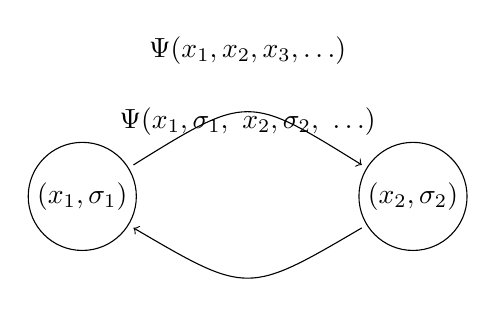
\begin{tikzpicture}
\node at (0,1.65) {$\Psi(x_1,x_2,x_3,\ldots)$};
\node at (0,0.75) {$\Psi(x_1,\sigma_1,\ x_2,\sigma_2,\ \ldots)$};

\node[draw,circle,inner sep=2pt] (a) at (-2.1,-0.2) {$(x_1,\sigma_1)$};
\node[draw,circle,inner sep=2pt] (b) at (2.1,-0.2) {$(x_2,\sigma_2)$};

\draw[->] (-1.45,0.2) .. controls (0,1.1) .. (1.45,0.2);
\draw[->] (1.45,-0.6) .. controls (0,-1.45) .. (-1.45,-0.6);
\end{tikzpicture}
\end{figure}

Thus the exchange rule becomes
\begin{align}
\psi_B(x_1,\sigma_1;\,x_2,\sigma_2)
&=+\psi_B(x_2,\sigma_2;\,x_1,\sigma_1), \\
\psi_F(x_1,\sigma_1;\,x_2,\sigma_2)
&=-\psi_F(x_2,\sigma_2;\,x_1,\sigma_1).
\end{align}
What follows is exactly the statement with which the lecture began: two fermions cannot occupy the same full state, including spin. Two electrons may therefore share the same spatial orbital only when their spin labels differ.

A student remarks that this sounds like the permutation group, and Susskind agrees completely. Exchange is a permutation, and the \(\pm1\) behavior furnishes a one-dimensional representation of the permutation group. In a compact operator notation one may write
\begin{equation}
P_{12}\psi_{\pm}=\pm \psi_{\pm},
\end{equation}
but the lecture's real point is the explicit one: exchange acts on the entire particle label.

Another student asks about the difference between adding wavefunctions and multiplying them. Susskind uses the question to separate two ideas that are often muddled. If one adds one-particle wavefunctions,
\begin{equation}
\alpha\,\psi_0+\beta\,\psi_1,
\end{equation}
one is describing a single particle in a superposition of two states. If instead one writes
\begin{equation}
\psi_0(x_1)\psi_1(x_2),
\end{equation}
one is building a two-particle product state: particle \(1\) in one state, particle \(2\) in the other. Symmetrization or antisymmetrization comes only after that product has been formed.

The student discussion also foreshadows something Susskind will return to later. Because the same-state fermionic construction vanishes by cancellation of amplitudes, the Pauli principle can be viewed as a peculiar interference phenomenon. At this stage he leaves that remark hanging and turns to the second minus sign.

\section{Rotation by \(2\pi\) and the Second Minus Sign}

The first minus sign concerned exchange of two identical fermions. The second concerns a single particle with half-integer angular momentum. Susskind asks what happens if one rotates a state by an angle \(\theta\), in particular by a full \(2\pi\).

At first sight one expects nothing at all. A \(2\pi\) rotation is geometrically the identity rotation. But the same loophole that appeared in the exchange discussion appears here too: if all that must remain unchanged are probabilities and expectation values, the state may return only up to a phase.

Let \(\psi(\theta)\) denote the state after a rotation by angle \(\theta\) about the \(z\)-axis. The generator of such rotations is \(J_z\). In Susskind's convention,
\begin{equation}
J_z\,\psi(\theta)=-i\,\frac{\partial}{\partial\theta}\psi(\theta).
\end{equation}
Now suppose the state is a \(J_z\)-eigenstate with eigenvalue \(m\):
\begin{equation}
J_z\,\psi=m\,\psi.
\end{equation}
Combining the two equations gives
\begin{equation}
-i\,\frac{\partial}{\partial\theta}\psi(\theta)=m\,\psi(\theta),
\end{equation}
whose solution is
\begin{equation}
\psi(\theta)=e^{im\theta}\psi(0).
\end{equation}
Therefore
\begin{equation}
\psi(2\pi)=e^{i2\pi m}\psi(0).
\end{equation}

At this point the lecture appeals to the familiar spectrum of angular momentum. The eigenvalues of \(J_z\) are either integers or half-integers. Hence
\begin{equation}
m\in\mathbb{Z}
\quad\Rightarrow\quad
e^{i2\pi m}=+1,
\end{equation}
while
\begin{equation}
m\in\mathbb{Z}+\frac12
\quad\Rightarrow\quad
e^{i2\pi m}=-1.
\end{equation}
Integer-spin states therefore return to themselves under \(2\pi\), while half-integer-spin states return with a minus sign. A \(4\pi\) rotation restores all of them:
\begin{equation}
\psi(4\pi)=\psi(0).
\end{equation}

This is the second minus sign of the lecture. It has nothing directly to do with exchanging two particles. It belongs already to the rotational behavior of a single half-integer-spin state.

\begin{remark}
For notational cleanliness one may also write the rotation operator in the standard form
\begin{equation}
R_z(\theta)=e^{-i\theta J_z}.
\end{equation}
The lecture itself proceeds instead through the differential relation \(J_z=-i\,\partial/\partial\theta\) acting on \(\psi(\theta)\). Because of this, one should not overemphasize the sign convention in the exponent. The physical invariant is the behavior under \(2\pi\): integer spin gives \(+1\), half-integer spin gives \(-1\), and \(4\pi\) gives the identity.
\end{remark}

Susskind immediately adds an important warning. The minus sign acquired under a \(2\pi\) rotation is not itself visible in ordinary probabilities, any more than the exchange sign was. But that does not mean it is mathematically trivial. It is not the identity operation for fermions, only an operation whose effect disappears in \(|\psi|^2\).

\section{Topology, Spin-Statistics, and Observability}

At this stage the lecture becomes more heuristic. Susskind shifts from algebra to pictures, demonstrations, and topology. He is not giving Pauli's rigorous proof of the spin-statistics theorem. He is trying to show why the two minus signs do not merely resemble one another accidentally.

\paragraph{The \(4\pi\) topology.}

The cup trick and the belt trick are used to exhibit a basic fact about the topology of the rotation group. A path in rotation space corresponding to a \(2\pi\) rotation is nontrivial; a path corresponding to \(4\pi\) can be unwound. In Susskind's language, a \(2\pi\) twist gives a tangle, while after another \(2\pi\) the tangle can be undone. This is why the mathematics naturally distinguishes \(2\pi\) from \(4\pi\).

The lesson is not yet spin-statistics. It is only that the half-integer behavior under \(2\pi\) is not a cheap artifact of notation. It reflects the topology of the rotation group in three dimensions.

\paragraph{Exchange plus \(2\pi\) rotation.}

The lecture then takes a more suggestive step. Susskind attributes to David Finkelstein a deeper topological observation: exchange of two particles and a \(2\pi\) rotation of one particle are related. The belt demonstration makes this vivid. A belt configuration that can be read one way as an exchange can be read another way as a \(2\pi\) twist, and ``exchange plus a \(2\pi\) rotation'' becomes topologically trivial.

He then translates the picture into a worldline-type argument. Begin with no particles. Create two particle-antiparticle pairs, so that at an intermediate time there are four particles present. Now rotate one of them by \(2\pi\) and simultaneously exchange two of the others. Topologically, Susskind argues, this history can be deformed into a trivial creation-annihilation process. A trivial process should carry no net phase. Therefore the phase acquired from exchange must cancel the phase acquired from rotation.

That is the lecture's heuristic version of the spin-statistics link. It is not presented as a proof, and Susskind explicitly says he has never seen it turned into a fully rigorous derivation in the form he likes. But it captures the right moral: the exchange sign and the \(2\pi\) rotation sign are deeply connected, not merely parallel curiosities.

This is also why he broadens the discussion beyond elementary relativistic particles. Once the real criterion is the ability to create and annihilate particle-like excitations, the argument should apply equally to solitons, solitary waves, monopoles, and other lump-like excitations in field theory or condensed matter systems. In that sense he takes the topology to be closer to the root of spin-statistics than the specific historical proof.

\paragraph{Why a global sign is invisible.}

Susskind then asks the operational question: can one observe the minus sign from a \(2\pi\) rotation? If one rotates a single trapped electron adiabatically through \(2\pi\) and then compares it with an otherwise identical experiment in which no such rotation was performed, the answer is no. The phase change is only global. Since probabilities depend on \(\psi\psi^\ast\), the sign disappears.

This is the null experiment with which he begins the final part of the lecture. It is important because it prevents confusion. A universal \(2\pi\) rotation of everything is not what one measures. The measurable effect appears only when one compares two coherent branches relative to one another.

\paragraph{Relative phase from branch interference.}

Now take one electron and split its wavefunction coherently into two branches. In the lecture these are called \(\psi_1\) and \(\psi_2\); to avoid conflict with the earlier one-particle orbitals, let us write them as \(\psi_{\mathrm{L}}\) and \(\psi_{\mathrm{R}}\):
\begin{equation}
\psi(x)=\psi_{\mathrm{L}}(x)+\psi_{\mathrm{R}}(x).
\end{equation}
This is still one electron. One branch of its wavefunction goes one way, the other branch another way. If one looks to determine which branch the electron took, the interference is destroyed; that is precisely the ordinary two-slit logic that Susskind repeatedly invokes.

Now let only one branch execute a \(2\pi\) spin rotation, while the other branch is left alone. Then the state becomes
\begin{equation}
\psi(x)\longrightarrow \psi_{\mathrm{L}}(x)-\psi_{\mathrm{R}}(x).
\end{equation}
This minus sign is no longer global. It is a relative phase between coherent branches, and therefore it changes the interference pattern when the branches are brought back together. Constructive interference can become destructive interference, and a point of reinforcement can become a node.

That is the core observability argument. A \(2\pi\) rotation is unobservable as a global phase, but observable as a relative phase. Susskind then describes a more realistic version of the experiment: one sends a coherent electron beam through two arms, arranges a magnetic field in only one arm, and uses spin precession to make the spin in that arm execute one \(2\pi\) rotation while the other arm does not. The pure adiabatic version and the practical precession-based version differ in apparatus, but not in conceptual content.

He closes this part with a subtlety. What is being detected is not a literal \(2\pi\) rotation of the whole world. If the entire universe were rotated, no relative phase would be created and nothing observable would happen. The measurement works only because one branch of the world is rotated relative to another.

\paragraph{An exchange-interference coda.}

Right at the end, Susskind sketches a two-electron analog. One could imagine coherently splitting a pair of electrons into two branches, exchanging the electrons in one branch but not in the other, and then recombining the branches. The exchange sign would then appear as a relative phase, just as the \(2\pi\) rotation sign did in the one-electron interferometer. He even suggests a hybrid experiment in which exchange occurs on one branch and a \(2\pi\) rotation on the other, so that the two effects should cancel. The discussion remains exploratory, and he does not claim that such an experiment has been carried out. But it reinforces the final conceptual point: quantum indistinguishability is subtler than classical sameness, and the exchange sign is a real ingredient of interference.

\section{Summary}

The lecture proceeds deliberately from chemistry to abstraction. It begins by recalling that, in the old shell picture, state includes spin, so two electrons can share the lowest spatial orbital only when their spin labels differ. That empirical reminder sets up the real subject: the exclusion principle is encoded in the symmetry of many-particle wavefunctions. Bosons have symmetric wavefunctions, fermions antisymmetric ones, and the Pauli principle appears because the antisymmetric same-state combination vanishes. After spin is restored as part of the particle label, the same rule says that two fermions cannot occupy the same full state, including spin. Only then does Susskind introduce the second minus sign, the \(-1\) acquired by half-integer-spin states under a \(2\pi\) rotation. The final topological and interferometric arguments are deliberately suggestive rather than formal, but they leave the intended impression: exchange and \(2\pi\) rotation are deeply linked, and the sign picked up by a fermion under \(2\pi\) becomes physically visible whenever it is converted from a global phase into a relative one.